\chapter{Cơ sở lý thuyết}
\label{chap:theory}

Chương này trình bày các kiến thức nền tảng cần thiết để hiểu phương pháp PhaBERT-CNN được đề xuất trong luận văn. Nội dung được tổ chức thành bốn phần chính: (1) các khái niệm sinh học phân tử và tin sinh học bao gồm DNA, gen, thực khuẩn thể, siêu hệ gen và siêu hệ gen virus; (2) nền tảng học máy và học sâu gồm mạng nơ-ron tích chập, Transformer, BERT và các chỉ số đánh giá hiệu năng; (3) tổng quan về học chuyển giao trong tin sinh học; và (4) tổng quan các công trình liên quan về phân loại hệ gen phage.

% =====================================================================
\section{Nền tảng sinh học phân tử và tin sinh học}
\label{sec:bio_foundation}

\subsection{DNA, gen và bộ gen}
\label{subsec:dna_gene}

Axit deoxyribonucleic (DNA) là phân tử mang thông tin di truyền của hầu hết các sinh vật sống và nhiều loại virus. Năm 1953, Watson và Crick xác định rằng DNA có cấu trúc dạng xoắn kép, bao gồm hai chuỗi polynucleotide liên kết bổ sung chạy ngược chiều nhau~\cite{watson1953molecular}. Mỗi nucleotide bao gồm một phân tử đường deoxyribose, một nhóm phosphate, và một trong bốn bazơ nitơ: adenine (A), thymine (T), guanine (G), và cytosine (C). Theo nguyên tắc bổ sung Chargaff, A luôn ghép cặp với T và G luôn ghép cặp với C. Trật tự sắp xếp của bốn ký tự nucleotide dọc theo chuỗi DNA mã hóa toàn bộ thông tin di truyền của sinh vật, tạo thành cơ sở cho biểu diễn chuỗi hệ gen trong tin sinh học.

Gen là đơn vị cơ bản của thông tin di truyền, một đoạn DNA mã hóa cho một sản phẩm chức năng, thông thường là protein thông qua quá trình phiên mã (DNA sang RNA) rồi dịch mã (RNA sang chuỗi axit amin). Bộ gen là toàn bộ vật liệu di truyền của một sinh vật, bao gồm tất cả các gen và các vùng DNA không mã hóa. Kích thước bộ gen biến thiên rất lớn giữa các loài: từ vài kilobase (kb) ở các virus nhỏ đến hàng tỷ cặp bazơ (bp) ở sinh vật bậc cao. Đối với thực khuẩn thể, bộ gen có thể là DNA hoặc RNA, dạng sợi đơn hoặc sợi kép, với kích thước dao động từ dưới 10~kb ở các thực khuẩn thể nhỏ đến hơn 600~kb ở một số thực khuẩn thể lớn~\cite{brussow2002phage}. Đặc biệt, các nghiên cứu metagenomics gần đây đã phát hiện hàng trăm thực khuẩn thể với bộ gen vượt 200~kb, bao gồm các \textit{huge phage} với bộ gen ghi nhận lên đến 735~kb~\cite{al2020huge}. Sự đa dạng về kích thước và thành phần nucleotide (tỷ lệ GC) của bộ gen thực khuẩn đặt ra thách thức đáng kể cho các phương pháp phân tích dựa trên thống kê thành phần chuỗi.

\subsection{Thực khuẩn thể và phân loại hệ gen}
\label{sec:bacteriophage}

Thực khuẩn thể (bacteriophage), hay gọi tắt là phage, là các virus có khả năng xâm nhiễm và nhân lên bên trong tế bào vi khuẩn. Thực khuẩn thể được xem là dạng thực thể sinh học phong phú nhất trên Trái Đất, với số lượng ước tính vượt $10^{30}$ cá thể chỉ riêng trong môi trường đại dương~\cite{suttle2007marine}, và hiện diện ở hầu hết mọi môi trường có vi khuẩn sinh sống. Thực khuẩn thể đóng vai trò thiết yếu trong sinh thái vi sinh vật thông qua việc điều hòa quần thể vi khuẩn, đồng thời là tác nhân trung gian quan trọng trong quá trình chuyển gen ngang giữa các vi khuẩn~\cite{koskella2014bacteria}.

Dựa trên chiến lược nhân lên, thực khuẩn thể được phân loại thành hai nhóm chính~\cite{mcnair2012phacts,wu2021deephage}. Thực khuẩn thể độc lực chỉ thực hiện chu trình tan. Sau khi xâm nhiễm, thực khuẩn thể độc lực chiếm đoạt bộ máy tổng hợp của tế bào chủ để nhân bản hệ gen và tổng hợp các thành phần cấu trúc, lắp ráp thành các hạt virus con, rồi phá vỡ tế bào vi khuẩn để giải phóng thế hệ thực khuẩn thể mới. Thực khuẩn thể ôn hòa có khả năng thực hiện cả chu trình tan lẫn chu trình tiềm tan. Trong chu trình tiềm tan, DNA thực khuẩn được tích hợp vào nhiễm sắc thể vi khuẩn thông qua quá trình tái tổ hợp đặc hiệu vị trí được xúc tác bởi enzyme integrase, trở thành prophage. Prophage tồn tại ở trạng thái im lặng và được nhân lên cùng với hệ gen vi khuẩn qua nhiều thế hệ~\cite{howard2017lysogeny}. Khi tế bào chủ tiếp xúc với các tác nhân gây tổn thương ADN như bức xạ tử ngoại (UV), prophage có thể được cảm ứng, tách ra khỏi nhiễm sắc thể vi khuẩn và chuyển sang thực hiện chu trình tan~\cite{howard2017lysogeny}.

Việc phân loại chính xác hệ gen thực khuẩn có ý nghĩa thực tiễn quan trọng trong nhiều lĩnh vực ứng dụng. Trong liệu pháp sử dụng thực khuẩn để điều trị các bệnh nhiễm khuẩn kháng kháng sinh~\cite{gordillo2019phage}, chỉ thực khuẩn thể độc lực mới được xem là phù hợp vì chúng tiêu diệt vi khuẩn hiệu quả mà không tích hợp vào hệ gen tế bào chủ~\cite{gordillo2019phage,kortright2019phage}. Ngược lại, thực khuẩn thể ôn hòa tiềm ẩn nguy cơ truyền các gen độc lực hoặc gen kháng kháng sinh sang vi khuẩn bệnh nguyên thông qua biến đổi tiềm tan~\cite{brussow2004phages}.

Tuy nhiên, xác định hệ gen thực khuẩn bằng phương pháp thực nghiệm truyền thống đòi hỏi nuôi cấy và phân lập thực khuẩn trong phòng thí nghiệm, một quá trình tốn nhiều thời gian, chi phí cao và không khả thi với phần lớn các thực khuẩn chưa được nuôi cấy trong các mẫu môi trường~\cite{shang2023phatyp}. Điều này thúc đẩy sự phát triển của các phương pháp tính toán để dự đoán hệ gen thực khuẩn trực tiếp từ dữ liệu di truyền, đặc biệt trong bối cảnh metagenomics nơi hệ gen thực khuẩn thường thu được dưới dạng các contig ngắn và phân mảnh.

\subsection{Dữ liệu metagenomics và bài toán phân loại trên contig}
\label{sec:metagenomics}

Metagenomics (siêu hệ gen hay hệ gen môi trường) là lĩnh vực nghiên cứu vật liệu di truyền được thu thập trực tiếp từ các mẫu môi trường, cho phép phân tích toàn bộ cộng đồng vi sinh vật mà không cần nuôi cấy từng loài riêng lẻ~\cite{mokili2012metagenomics}. Phương pháp này đặc biệt quan trọng vì phần lớn vi sinh vật trong tự nhiên không thể nuôi cấy trong điều kiện phòng thí nghiệm. Một nhánh chuyên biệt gọi là \textit{viral metagenomics} (hay \textit{metaviromics}) tập trung vào thành phần virus trong mẫu môi trường. Dữ liệu thu được từ metaviromics cung cấp cái nhìn toàn diện về sự đa dạng và phân bố của các cộng đồng phage trong nhiều hệ sinh thái khác nhau, từ đại dương, đất đến ruột người~\cite{emerson2012dynamic,hayes2017metagenomic}. Chính nhờ đó, phần lớn sự đa dạng của thực khuẩn thể trong tự nhiên mới được hé lộ, trong khi các phương pháp phân lập truyền thống chỉ tiếp cận được một phần nhỏ quần thể virus thực sự tồn tại trong môi trường~\cite{mokili2012metagenomics}.

Trong phân tích siêu hệ gen (metagenomics), dữ liệu thô từ giải trình tự thế hệ mới là các đoạn đọc ngắn gọi là \textit{read}, mỗi read thường có độ dài từ vài chục đến vài trăm cặp bazơ tùy công nghệ sử dụng. Các đoạn đọc này được lắp ráp lại bằng thuật toán lắp ráp trình tự dựa trên vùng chồng lấp giữa chúng, tạo thành các đoạn trình tự dài hơn gọi là \textit{contig} (trình tự liên tục)~\cite{ghurye2016metagenomic}. Contig đại diện cho một vùng liên tục của bộ gen được tái tạo từ dữ liệu trình tự, song thường chưa đầy đủ do độ phủ không đồng đều, các vùng lặp lại, hoặc sai số kỹ thuật. Ở mức độ lắp ráp cao hơn, các contig được sắp xếp và định hướng tương đối với nhau dựa trên thông tin đọc ghép đôi đầu (paired-end reads) hoặc đọc dài (long reads), tạo thành \textit{scaffold}; khoảng cách giữa các contig trong scaffold thường được điền bằng ký tự ``N'' để biểu thị vùng trình tự chưa xác định~\cite{setubal2021metagenome}. Chuỗi phân cấp từ đoạn đọc, contig, scaffold đến bộ gen hoàn chỉnh phản ánh mức độ đầy đủ ngày càng tăng của dữ liệu trình tự thu được (Hình~\ref{fig:assembly_hierarchy}).

\begin{figure}[h]
  \centering
  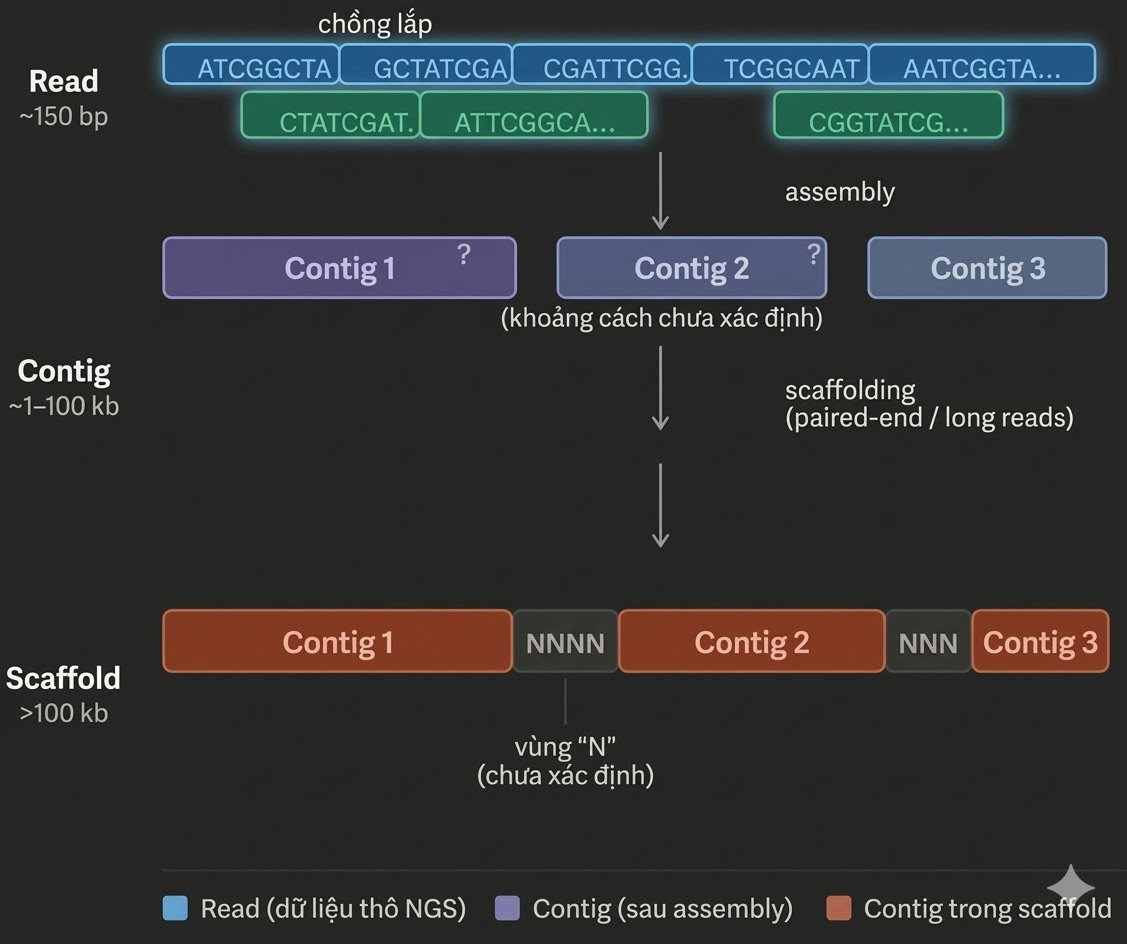
\includegraphics[width=0.9\textwidth]{imgs/hierachy_contig.png}
  \caption{Chuỗi phân cấp lắp ráp hệ gen từ read, contig, scaffold đến bộ gen hoàn chỉnh}
  \label{fig:assembly_hierarchy}
\end{figure}

Trong bối cảnh dự đoán hệ gen thực khuẩn thể, phần lớn dữ liệu đầu vào thực tế tồn tại ở dạng contig, các đoạn bộ gen không hoàn chỉnh với độ dài và mức độ đại diện rất khác nhau. Để đánh giá hiệu năng trên các contig có độ dài điển hình trong dữ liệu metavirome, các nghiên cứu DeePhage~\cite{wu2021deephage} và PhaTYP~\cite{shang2023phatyp} đã thống nhất sử dụng bốn nhóm độ dài: Nhóm~A (100--400~bp), Nhóm~B (400--800~bp), Nhóm~C (800--1200~bp), và Nhóm~D (1200--1800~bp). Nhóm~A bao phủ độ dài điển hình của các read thô từ giải trình tự Illumina (thường 75--300~bp); Nhóm~B--C bao phủ phần lớn contig ngắn thường gặp sau lắp ráp; và Nhóm~D đại diện cho các contig trung bình vẫn còn phân mảnh so với bộ gen phage hoàn chỉnh (thường 15--200~kb). Nghiên cứu này kế thừa cùng phân chia nhóm độ dài để đảm bảo khả năng so sánh trực tiếp với các phương pháp tiền nhiệm.

Các contig ngắn, đặc biệt dưới 400~bp, đặt ra thách thức đặc biệt cho phân loại bởi chúng thường không chứa gen hoàn chỉnh, khiến các công cụ dự đoán gen như Prodigal hoặc các công cụ tương đương giảm độ chính xác đáng kể trên các đoạn DNA ngắn có chứa lỗi giải trình tự~\cite{trimble2012short}. Đây là một trong những động lực chính cho việc phát triển các phương pháp học sâu hoạt động trực tiếp trên chuỗi DNA thô thay vì dựa vào đặc trưng protein, điển hình như mô hình PhaBERT-CNN được đề xuất trong luận văn này.

% =====================================================================
\section{Các phương pháp tính toán cho phân loại lối sống thực khuẩn}
\label{subsec:phage_classification_methods}

Nhận thức được tầm quan trọng của bài toán phân loại lối sống thực khuẩn, nhiều phương pháp tính toán đã được phát triển, từ các kỹ thuật học máy truyền thống đến các mô hình học sâu hiện đại và các mô hình nền tảng hệ gen. Phần này trình bày tổng quan các công trình liên quan, tổ chức theo sự phát triển của phương pháp luận: từ học máy truyền thống dựa trên đặc trưng thủ công, đến học sâu với khả năng tự động học biểu diễn, và cuối cùng là các mô hình nền tảng tận dụng học chuyển giao từ kho ngữ liệu hệ gen quy mô lớn.

\subsubsection{Các phương pháp học máy truyền thống}

Các phương pháp học máy truyền thống như PHACTS~\cite{mcnair2012phacts}, PhageAI~\cite{tynecki2020phageai}, và BACPHLIP~\cite{hockenberry2021bacphlip} đạt hiệu năng cao trên bộ gen thực khuẩn hoàn chỉnh, với độ chính xác thường vượt 90\%. Tuy nhiên, các phương pháp này được thiết kế và tối ưu hóa cho bộ gen hoàn chỉnh, do đó gặp khó khăn đáng kể khi áp dụng cho dữ liệu contig phân mảnh từ metagenomics.

\textbf{PHACTS}~\cite{mcnair2012phacts} sử dụng thuật toán Random Forest kết hợp với đặc trưng tương đồng protein. Phương pháp mã hóa dữ liệu của PHACTS gồm hai bước: (1) tạo tập protein chuẩn có chú thích lối sống, và (2) mã hóa proteome của thực khuẩn cần phân loại thành vector tương đồng thông qua công cụ FASTA35, so sánh với tập protein chuẩn, sau đó nối các vector tương đồng này để tạo vector mã hóa cuối cùng. PHACTS đạt độ chính xác cao trên bộ gen hoàn chỉnh (xấp xỉ 90\%), nhưng hiệu năng giảm mạnh trên contig ngắn---chỉ đạt khoảng 50\% độ chính xác trên các đoạn contig trong khoảng 100--1800~bp~\cite{wu2021deephage}, tương đương với dự đoán ngẫu nhiên. Nguyên nhân là các contig ngắn thiếu vùng mã hóa protein hoàn chỉnh để tạo tín hiệu tương đồng đủ tin cậy.

\textbf{PhageAI}~\cite{tynecki2020phageai} ứng dụng kỹ thuật xử lý ngôn ngữ tự nhiên cho dữ liệu di truyền, sử dụng phân tách k-mer để chuyển đổi chuỗi DNA thành định dạng văn bản, sau đó áp dụng Word2Vec để tạo biểu diễn embedding đặc trưng. Nguồn dữ liệu của PhageAI là bộ gen thực khuẩn hoàn chỉnh. Phương pháp này sử dụng Recursive Feature Elimination with Cross-Validation (RFECV) để loại bỏ các đặc trưng dư thừa, chỉ giữ lại những đặc trưng có ảnh hưởng đáng kể đến hiệu năng phân loại. Thuật toán máy vector hỗ trợ (Support Vector Machine --- SVM) được sử dụng cho phân loại và cho kết quả tốt nhất. PhageAI đạt độ chính xác cao trên bộ gen hoàn chỉnh, tuy nhiên bị hạn chế trên contig ngắn do tín hiệu ngữ cảnh không đủ để Word2Vec học được biểu diễn có ý nghĩa.

\textbf{BACPHLIP}~\cite{hockenberry2021bacphlip} khai thác sự hiện diện của các protein bảo tồn liên quan đến chu kỳ tiềm tan. Nguồn dữ liệu là bộ gen thực khuẩn hoàn chỉnh. Phương pháp mã hóa của BACPHLIP gồm hai bước: (1) nhận diện các vùng protein bảo tồn thông qua công cụ HMMER3, và (2) tạo vector đặc trưng nhị phân biểu diễn sự hiện diện của các vùng bảo tồn này. Thuật toán Random Forest được sử dụng cho phân loại và cho hiệu năng cạnh tranh. Tuy nhiên, sự khan hiếm dữ liệu về các vùng protein bảo tồn gây khó khăn cho ứng dụng thực tế. Theo khuyến nghị của tác giả, BACPHLIP chỉ phù hợp với bộ gen hoàn chỉnh và trả về kết quả lỗi khi nhận đầu vào là contig phân mảnh~\cite{shang2023phatyp}.

\subsubsection{Các phương pháp học sâu}

Sự phát triển của công nghệ tính toán song song đã cho phép phát triển và công bố các mô hình học sâu tinh vi như DeePhage~\cite{wu2021deephage}, PhaTYP~\cite{shang2023phatyp}, DeepPL~\cite{zhang2024deeppl}, và ProkBERT~\cite{ligeti2024prokbert}. Các tiến bộ công nghệ này dẫn đến cải thiện dần hiệu năng phân loại, đặc biệt trên dữ liệu contig phân mảnh, làm cho phân loại thực khuẩn bằng tính toán ngày càng khả thi cho các ứng dụng thực tế.

\textbf{DeePhage}~\cite{wu2021deephage} là phương pháp học sâu đầu tiên được đề xuất cho bài toán phân loại lối sống phage trên dữ liệu metagenomics. Nguồn dữ liệu của DeePhage là các contig metagenomic với độ dài từ 100 đến 1800~bp, được chia thành bốn nhóm: Nhóm~A (100--400~bp), Nhóm~B (400--800~bp), Nhóm~C (800--1200~bp), và Nhóm~D (1200--1800~bp). Phương pháp phân tách token của DeePhage là mã hóa one-hot trực tiếp trên chuỗi DNA thô, trong đó mỗi nucleotide được mã hóa thành vector nhị phân 4 chiều: A~=~[0,0,0,1], C~=~[0,0,1,0], G~=~[0,1,0,0], T~=~[1,0,0,0]. Thuật toán sử dụng là mạng nơ-ron tích chập (CNN) được huấn luyện từ đầu (from scratch) mà không sử dụng huấn luyện trước. DeePhage không phụ thuộc vào dự đoán gen, có khả năng xử lý contig ngắn, đạt độ chính xác kiểm định chéo 5 lần lên đến 89\%---vượt trội so với PHACTS và PhagePred lần lượt khoảng 30\% và 10\%---đồng thời nhanh hơn 810 lần về thời gian tính toán so với PHACTS~\cite{wu2021deephage}. Bộ chuẩn đánh giá gồm bốn nhóm độ dài contig A--D do DeePhage thiết lập cũng được sử dụng rộng rãi trong các nghiên cứu tiếp theo. Hạn chế chính của DeePhage là mô hình được huấn luyện từ đầu mà không tận dụng được tri thức hệ gen tổng quát từ kho ngữ liệu lớn, và mã hóa one-hot tạo ra biểu diễn thưa (sparse) không mang thông tin ngữ nghĩa.

\textbf{PhaTYP}~\cite{shang2023phatyp} là phương pháp đầu tiên ứng dụng kiến trúc BERT cho bài toán phân loại lối sống phage. Nguồn dữ liệu của PhaTYP là bộ gen thực khuẩn hoàn chỉnh và contig. Phương pháp phân tách token của PhaTYP hoạt động ở cấp độ protein: genome thực khuẩn được dịch mã thành các protein thông qua công cụ dự đoán gen Prodigal~\cite{hyatt2010prodigal}, sau đó các protein đồng nhất được nhóm lại thành các cluster, mỗi cluster được coi là một token. Mỗi genome thực khuẩn được coi là một "câu" gồm các token là protein cluster. Thuật toán sử dụng là BERT (Transformer encoder) được huấn luyện trước bằng học tự giám sát trên chuỗi protein, sau đó tinh chỉnh cho tác vụ phân loại lối sống. PhaTYP đạt hiệu năng mạnh trên contig dài, đặc biệt là Nhóm~D (1200--1800~bp) với 92.29\% độ nhạy, 89.75\% độ đặc hiệu, và 91.02\% độ chính xác. Tuy nhiên, PhaTYP phụ thuộc vào bước dự đoán gen trung gian---Prodigal vốn có hiệu suất giảm mạnh trên các đoạn DNA ngắn hơn 200~bp~\cite{trimble2012short}---dẫn đến hạn chế đáng kể trên contig ngắn và phân mảnh~\cite{shang2023phatyp}.

\textbf{DeepPL}~\cite{zhang2024deeppl} sử dụng DNABERT~\cite{ji2021dnabert} để mã hóa chuỗi DNA cho phân loại lối sống phage. Nguồn dữ liệu là các contig metagenomic. Phương pháp phân tách token của DeepPL là k-mer có chồng lấp (overlapping k-mer), thường với $k=6$, trong đó các token liền kề chia sẻ $k-1$ nucleotide. Thuật toán sử dụng là DNABERT, một mô hình BERT được huấn luyện trước trên hệ gen người. DeepPL không phụ thuộc vào dự đoán gen, hoạt động trực tiếp trên chuỗi DNA. Tuy nhiên, DeepPL kế thừa hạn chế của DNABERT gốc về giới hạn độ dài chuỗi tối đa 512 token do sử dụng biểu diễn vị trí học được (learned positional embedding)~\cite{ji2021dnabert}---tương đương khoảng 500~bp với $k=6$. Do hạn chế này, DeepPL không thể xử lý contig dài hơn trong bộ chuẩn của nghiên cứu (lên đến 1800~bp) và do đó bị loại khỏi so sánh trực tiếp. Ngoài ra, phân tách k-mer có chồng lấp gây ra hiện tượng rò rỉ thông tin trong quá trình học có mặt nạ và kém hiệu quả tính toán do số token xấp xỉ độ dài chuỗi gốc.

\textbf{ProkBERT}~\cite{ligeti2024prokbert} là họ mô hình ngôn ngữ hệ gen vi sinh. Nguồn dữ liệu huấn luyện trước là hệ gen vi khuẩn đa loài. Phương pháp phân tách token của ProkBERT sử dụng cơ chế nhận thức ngữ cảnh cục bộ (Local Context-Aware --- LCA)---một biến thể k-mer có chồng lấp với độ dịch chuyển điều chỉnh được, cho phép mở rộng ngữ cảnh mà không làm tăng đáng kể chi phí tính toán. Thuật toán sử dụng là BERT được huấn luyện trước trên kho ngữ liệu hệ gen vi sinh đa loài. ProkBERT đạt hiệu năng trung bình trên bộ chuẩn phân loại phage, với độ chính xác dao động từ 80.68\% đến 85.35\%. Đáng chú ý, khác với các phương pháp khác có xu hướng cải thiện đều đặn khi độ dài contig tăng, ProkBERT cho thấy hiện tượng trì trệ hiệu năng trên contig dài hơn, với độ chính xác đạt đỉnh 85.35\% ở Nhóm~B rồi giảm xuống khoảng 84\% ở Nhóm~C và D. Mẫu hiệu năng này gợi ý những hạn chế tiềm ẩn trong khả năng nắm bắt phụ thuộc dài hạn hoặc các mẫu chuỗi phức tạp có trong các đoạn hệ gen mở rộng. Do vẫn dựa trên k-mer có chồng lấp, LCA tokenization tiềm ẩn hiện tượng rò rỉ thông tin trong giai đoạn tiền huấn luyện tương tự DNABERT gốc~\cite{ji2021dnabert,ligeti2024prokbert}.

\subsubsection{Các mô hình nền tảng hệ gen}

Sự phát triển của các mô hình nền tảng hệ gen (genomic foundation models) đánh dấu bước tiến quan trọng trong phân tích chuỗi sinh học, cho phép tận dụng tri thức từ kho ngữ liệu hệ gen quy mô lớn thông qua học chuyển giao.

\textbf{DNABERT}~\cite{ji2021dnabert} là mô hình nền tảng đầu tiên áp dụng kiến trúc BERT cho phân tích chuỗi DNA. Nguồn dữ liệu huấn luyện trước là hệ gen người. Phương pháp phân tách token của DNABERT là k-mer có chồng lấp, thường với $k=6$, trong đó chuỗi DNA được chia thành các đoạn con liên tiếp độ dài $k$, các token liền kề chia sẻ $k-1$ nucleotide. Thuật toán sử dụng là BERT được huấn luyện trước với mục tiêu mô hình hóa ngôn ngữ có mặt nạ (masked language modeling) trên hệ gen người. DNABERT gặp ba hạn chế chính~\cite{zhou2023dnabert}: (1) rò rỉ thông tin---do các token liền kề chia sẻ $k-1$ nucleotide, mô hình có thể suy luận được nội dung của token bị che từ các token xung quanh, làm giảm hiệu quả học; (2) kém hiệu quả tính toán---số token xấp xỉ độ dài chuỗi gốc ($L - k + 1 \approx L$), dẫn đến chi phí tính toán cao; (3) giới hạn độ dài cứng 512 token do sử dụng biểu diễn vị trí học được, không thể ngoại suy sang chuỗi dài hơn.

\textbf{DNABERT-2}~\cite{zhou2023dnabert} là mô hình nền tảng hệ gen đa loài thế hệ mới, khắc phục các hạn chế của DNABERT thông qua ba cải tiến kiến trúc chính. Nguồn dữ liệu huấn luyện trước là kho ngữ liệu hệ gen đa loài bao gồm nhiều sinh vật khác nhau, với độ dài chuỗi trung bình khoảng 700 cặp bazơ. Phương pháp phân tách token của DNABERT-2 là Byte Pair Encoding (BPE)~\cite{sennrich2015neural} thông qua bộ khung SentencePiece~\cite{kudo2018sentencepiece}. BPE xây dựng từ điển 4.096 token bằng cách lặp lại việc ghép các cặp ký tự liền kề xuất hiện thường xuyên nhất trong kho ngữ liệu, tạo ra các token có độ dài thay đổi với độ dài trung bình khoảng 5 nucleotide, giảm độ dài chuỗi khoảng 5 lần so với DNABERT. BPE loại bỏ hoàn toàn rò rỉ thông tin vì các token không chồng lấp nhau, mỗi nucleotide chỉ thuộc về một token duy nhất. Ngoài ra, BPE biến đổi mô hình hóa ngôn ngữ có mặt nạ thành bài toán dự đoán đoạn (span prediction)---mô hình cần dự đoán cả số lượng nucleotide lẫn danh tính của chúng trong token bị che, được chứng minh giúp tăng hiệu quả học~\cite{zhou2023dnabert,raffel2020exploring}.

Thuật toán của DNABERT-2 là BERT với các cải tiến kiến trúc: (1) mã hóa vị trí ALiBi (Attention with Linear Biases)~\cite{press2021train} thay thế biểu diễn vị trí học được, cho phép xử lý chuỗi có độ dài tùy ý mà không cần huấn luyện lại; (2) tích hợp Flash Attention~\cite{dao2022flashattention} giúp giảm tiêu thụ bộ nhớ và tăng tốc huấn luyện, làm cho mô hình hiệu quả hơn 3 lần so với DNABERT trong khi chỉ sử dụng một phần ba số FLOPs mặc dù có nhiều hơn 30\% tham số. DNABERT-2 được huấn luyện trước với mục tiêu mô hình hóa ngôn ngữ có mặt nạ trên kho ngữ liệu đa loài.

Trên bộ chuẩn Genome Understanding Evaluation (GUE)---một tập dữ liệu toàn diện gồm 36 tác vụ thuộc 9 danh mục phân tích hệ gen với chuỗi có độ dài từ 70 đến 10.000~bp---DNABERT-2 đạt hiệu năng tương đương mô hình Nucleotide Transformer 2,5 tỉ tham số~\cite{dalla2025nucleotide} trong khi nhỏ hơn 21 lần và yêu cầu ít hơn khoảng 92 lần thời gian GPU trong quá trình huấn luyện trước. DNABERT-2 vượt trội DNABERT trên 23 trong số 28 tập dữ liệu thuộc bộ chuẩn GUE. Mô hình thể hiện hiệu năng ổn định trên các độ dài chuỗi khác nhau, xử lý hiệu quả các đầu vào ngắn hơn 10 lần hoặc dài hơn 15 lần so với những gì gặp trong quá trình huấn luyện trước.

\subsubsection{So sánh tổng hợp các phương pháp}

Bảng~\ref{tab:comprehensive_method_comparison} tổng hợp so sánh các phương pháp phân loại lối sống thực khuẩn theo các tiêu chí chính: nguồn dữ liệu, phương pháp phân tách token, thuật toán áp dụng, huấn luyện trước, và hiệu năng trên contig ngắn.

\begin{table}[h]
\centering
\caption{So sánh tổng hợp các phương pháp phân loại lối sống thực khuẩn}
\label{tab:comprehensive_method_comparison}
\resizebox{\textwidth}{!}{%
\begin{tabular}{lccccc}
\toprule
\textbf{Phương pháp} & \textbf{Nguồn dữ liệu} & \textbf{Phân tách token} & \textbf{Thuật toán} & \textbf{Huấn luyện trước} & \textbf{Contig ngắn} \\
\midrule
PHACTS~\cite{mcnair2012phacts} & Bộ gen hoàn chỉnh & Vector tương đồng protein & Random Forest & Không & Yếu ($\sim$50\%) \\
PhageAI~\cite{tynecki2020phageai} & Bộ gen hoàn chỉnh & Word2Vec (k-mer) & SVM & Có & Trung bình \\
BACPHLIP~\cite{hockenberry2021bacphlip} & Bộ gen hoàn chỉnh & Miền protein bảo tồn & Random Forest & Không & Yếu (lỗi) \\
DeePhage~\cite{wu2021deephage} & Contig (100--1800 bp) & Mã hóa one-hot & CNN & Không & Trung bình (89\%) \\
PhaTYP~\cite{shang2023phatyp} & Bộ gen và contig & Protein cluster & BERT & Có & Yếu (<200 bp) \\
DeepPL~\cite{zhang2024deeppl} & Contig & k-mer có chồng lấp & DNABERT & Có & Bị loại ($\leq$500 bp) \\
ProkBERT~\cite{ligeti2024prokbert} & Hệ gen vi sinh & LCA k-mer & BERT & Có & Trung bình (trì trệ) \\
\textbf{PhaBERT-CNN} & \textbf{Contig (100--1800 bp)} & \textbf{BPE} & \textbf{DNABERT-2 + CNN} & \textbf{Có} & \textbf{Tốt} \\
\bottomrule
\end{tabular}%
}
\end{table}

\subsubsection{Khoảng trống nghiên cứu và động lực}

Qua tổng quan các công trình liên quan, có thể xác định bốn khoảng trống nghiên cứu chính cần giải quyết trong phân loại lối sống thực khuẩn từ dữ liệu metagenomics:

\textbf{(1) Sự phụ thuộc vào dự đoán gen.} PhaTYP~\cite{shang2023phatyp} phụ thuộc vào Prodigal~\cite{hyatt2010prodigal} để phát hiện protein, dẫn đến thất bại trên contig ngắn vì các công cụ dự đoán gen có hiệu suất giảm mạnh trên các đoạn DNA ngắn hơn 200~bp~\cite{trimble2012short}. Các contig ngắn thường không chứa gen hoàn chỉnh, khiến phương pháp dựa trên protein không khả thi.

\textbf{(2) Rò rỉ thông tin từ phân tách k-mer có chồng lấp.} DNABERT~\cite{ji2021dnabert}, DeepPL~\cite{zhang2024deeppl}, và ProkBERT~\cite{ligeti2024prokbert} sử dụng phân tách k-mer có chồng lấp, trong đó các token liền kề chia sẻ $k-1$ nucleotide. Điều này gây ra rò rỉ thông tin trong quá trình học có mặt nạ---mô hình có thể suy luận được nội dung của token bị che từ các token xung quanh---làm giảm hiệu quả học~\cite{zhou2023dnabert}.

\textbf{(3) Giới hạn độ dài chuỗi.} DeepPL~\cite{zhang2024deeppl} kế thừa giới hạn 512 token của DNABERT gốc do sử dụng biểu diễn vị trí học được, tương đương khoảng 500~bp với $k=6$. Giới hạn này khiến DeepPL không thể xử lý contig dài hơn trong bộ chuẩn (lên đến 1800~bp).

\textbf{(4) Thiếu tri thức huấn luyện trước.} DeePhage~\cite{wu2021deephage} được huấn luyện từ đầu mà không tận dụng tri thức hệ gen từ huấn luyện trước trên kho ngữ liệu lớn. Điều này hạn chế khả năng tổng quát hóa của mô hình, đặc biệt khi phân tích các chuỗi không hoàn chỉnh với thông tin ngữ cảnh hạn chế.

PhaBERT-CNN được đề xuất nhằm giải quyết đồng thời cả bốn khoảng trống này: (1) hoạt động trực tiếp trên chuỗi DNA thô không cần dự đoán gen, (2) sử dụng DNABERT-2 với phân tách BPE loại bỏ rò rỉ thông tin, (3) tận dụng mã hóa vị trí ALiBi cho phép xử lý chuỗi có độ dài tùy ý, và (4) khai thác tri thức hệ gen từ huấn luyện trước đa loài của DNABERT-2 thông qua học chuyển giao. Ngoài ra, PhaBERT-CNN kết hợp kiến trúc CNN đa tỷ lệ để trích xuất đặc trưng cục bộ từ biểu diễn DNABERT-2 và cơ chế gộp chú ý để tổng hợp thông tin toàn cục, tạo ra một giải pháp toàn diện cho phân loại lối sống phage trên dữ liệu metagenomics.



% =====================================================================
\section{Học chuyển giao trong tin sinh học}
\label{sec:transfer_learning}

Học chuyển giao (transfer learning) là mô hình học máy trong đó tri thức thu được từ việc huấn luyện trên tác vụ hoặc kho ngữ liệu nguồn được tái sử dụng để cải thiện hiệu năng trên tác vụ mục tiêu với ít dữ liệu có nhãn hơn~\cite{pan2009survey,zhuang2021comprehensive}. Trong bối cảnh deep learning hiện đại, điều này thường được hiện thực hóa qua paradigm huấn luyện trước–tinh chỉnh (pretrain–fine-tune): mô hình được huấn luyện trước trên corpus lớn không nhãn, sau đó tinh chỉnh cho tác vụ cụ thể~\cite{devlin2019bert,howard2018universal}.

Có ba chiến lược tinh chỉnh chính. Trích xuất đặc trưng (feature extraction) đóng băng toàn bộ mạng nền (backbone) và chỉ huấn luyện các lớp đặc thù tác vụ, bảo toàn hoàn toàn tri thức huấn luyện trước nhưng hạn chế khả năng thích nghi. Tinh chỉnh toàn bộ (full fine-tuning) cập nhật toàn bộ tham số, cho phép thích nghi tối đa nhưng có nguy cơ quá khớp (overfitting) khi dữ liệu có nhãn ít. Tinh chỉnh phân biệt (discriminative fine-tuning)~\cite{howard2018universal} áp dụng tốc độ học khác nhau cho các nhóm tham số---tốc độ học thấp cho mạng nền để bảo toàn tri thức huấn luyện trước, tốc độ học cao hơn cho các lớp đặc thù tác vụ để thích nghi nhanh. Chiến lược này cân bằng giữa bảo toàn tri thức tổng quát và thích nghi đặc thù của bài toán.

Một thách thức quan trọng là quên thảm khốc (catastrophic forgetting)---hiện tượng mô hình quên tri thức đã học trong huấn luyện trước khi tinh chỉnh quá mạnh trên tác vụ cụ thể. Để giảm thiểu, các kỹ thuật như tốc độ học phân biệt, mở khóa dần dần (gradual unfreezing, dần mở khóa các lớp từ trên xuống dưới) và chính quy hóa (regularization: giảm trọng số, dropout) thường được kết hợp~\cite{howard2018universal}.